\section{General}\label{sec:general}
The software has the task to gather the image information from the camera, detecting the ball, predicting where it will go in the future and controlling the motors to either stop or shoot the ball.
This task can be split into the following chapters:
\begin{itemize}
    \item \textbf{Optics}: Correcting for Lens distortion and converting the pixel coordinates to real world coordinates
    \item \textbf{Ball Detection}: Detecting the ball in the image
    \item \textbf{Prediction}: Predicting the ball movement
    \item \textbf{Controlling the motors}: Finally, we move the motors to the correct position
\end{itemize}


\section{Optics}\label{sec:optics}
The goal here is to correct for lens distortion, this can be achieved by first capturing many images containing a checkerboard pattern with known gird size, in this is case 8x8.
One such image in my case looks like this:
\begin{figure}[H]
    \centering
    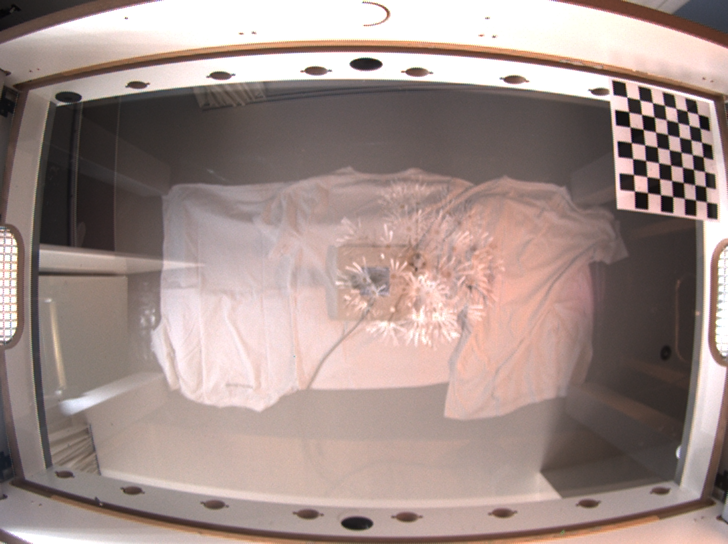
\includegraphics[height=5cm]{../photos/calibration_image}
    \caption[calimage]{Calibration image}
    \label{fig:calibration_image}
\end{figure}
As one can see there is severe distortion in the image, this can be corrected by using the OpenCV library.

% todo: should i explain in detail how opencv does it?
% lets do it and later i can delete it if its too much

\subsection{OpenCV}\label{subsec:opencv}
OpenCV is a library that provides many functions for image processing, one of these functions is the camera calibration function.
The function takes the images of the checkerboard pattern and calculates the distortion coefficients and the camera matrix.

The key principal is to map the distorted image to an undistorted image, this is done by calculating the pixel coordinates of the undistorted image for each pixel in the distorted image.
The Formulas for this are:
\begin{itemize}
    \item \textbf{Radial distortion:} This is the distortion that makes straight lines appear curved:
    \begin{gather*}
        r^2 = x^2 + y^2\\
        x_{\text{radial}} = x(1 + k_1 r^2 + k_2 r^4 + k_3 r^6)\\
        y_{\text{radial}} = y(1 + k_1 r^2 + k_2 r^4 + k_3 r^6)\\
    \end{gather*}
    \item \textbf{Tangential distortion:} This distortion occurs because the lens and the image sensor are not perfectly parallel.
    \begin{gather*}
        x_{\text{tangential}} = 2p_1 xy + p_2(r^2 + 2x^2)\\
        y_{\text{tangential}} = p_1(r^2 + 2y^2) + 2p_2 xy\\
    \end{gather*}
\end{itemize}
Together that gives:
\begin{gather*}
    x' = x_{\text{radial}} + x_{\text{tangential}}\\
    y' = y_{\text{radial}} + y_{\text{tangential}}\\
\end{gather*}
Finally, the undistorted pixel positions are transformed back to image coordinates using the camera matrix \( K \):
\[
    \begin{bmatrix}
        u \\
        v
    \end{bmatrix}
    =
    K \cdot
    \begin{bmatrix}
        x' \\
        y' \\
        1
    \end{bmatrix}
\]
where $K$ is the camera matrix:
\begin{center}
    K = \begin{bmatrix}
            f_x & 0   & c_x \\
            0   & f_y & c_y \\
            0   & 0   & 1
    \end{bmatrix}\\
    where:
\end{center}
\begin{itemize}
    \item $f_x$ and $f_y$ are the focal lengths along the x and y axes (in pixels),
    \item $c_x$ and $c_y$ are the coordinates of the optical center (principal point), typically at the center of the image.
\end{itemize}
These formulas allow the distorted image points to be remapped to undistorted coordinates.

\subsubsection{Implementation}\label{subsubsec:implementation}


Using the undistort function provided by opencv is not fast enough for our needs, because we only have 3ms to do the whole image processing and motor controlling.
So I wrote a custom function that generates a table where the index for each pixel in the new image is stored, so the function doesnt have to calculate the pixel coordinate for the undistorted image each time when the function is called.
The rust function to get the coordinates $x_{\text{original}},y_{\text{original}}$ of a pixel at $x_{\text{undistorted}},y_{\text{undistorted}}$ in the distorted (original) image looks like this:



\begin{lstlisting}[language=rust,breaklines,label={lst:distort_coords}]
/// Calculate the distorted coordinates given undistorted image coordinates.
fn distort_coords(x: f64, y: f64, fx: f64, fy: f64, cx: f64, cy: f64) -> (f64, f64) {
    // Distortion coefficients
    let k1 = DIST_COEFFS[0];
    let k2 = DIST_COEFFS[1];
    let p1 = DIST_COEFFS[2];
    let p2 = DIST_COEFFS[3];
    let k3 = DIST_COEFFS[4];

    // Normalize coordinates to [-1, 1]
    let x_normalized = (x - cx) / fx;
    let y_normalized = (y - cy) / fy;

    // Calculate radial distance
    let r2 = x_normalized * x_normalized + y_normalized * y_normalized;
    let r4 = r2 * r2;

    // Apply radial distortion
    let radial_distortion = 1.0 + k1 * r2 + k2 * r4 + k3 * r4 * r2;
    let x_radial = x_normalized * radial_distortion;
    let y_radial = y_normalized * radial_distortion;

    // Apply tangential distortion
    let x_tangential =
        2.0 * p1 * x_normalized * y_normalized + p2 * (r2 + 2.0 * x_normalized * x_normalized);
    let y_tangential =
        p1 * (r2 + 2.0 * y_normalized * y_normalized) + 2.0 * p2 * x_normalized * y_normalized;

    // Distorted coordinates
    let x_distorted = x_radial + x_tangential;
    let y_distorted = y_radial + y_tangential;

    // Map back to pixel coordinates
    let distorted_x = fx * x_distorted + cx;
    let distorted_y = fy * y_distorted + cy;

    (distorted_x, distorted_y)
}
\end{lstlisting}
Where \texttt{DIST\_COEFFS} are the distortion coefficients calculated by the OpenCV calibration function.
To generate the table I used the following code:
\begin{lstlisting}[language=rust,breaklines,label={lst:gen_table}]
/// Generate precomputation table for undistortion.
pub fn gen_table(
    original_width: u32, original_height: u32,
    new_width: u32, new_height: u32,
    x_offset: i32, y_offset: i32,
) -> Vec<i32> {
    // Camera matrix values
    let fx = CAMERA_MATRIX[0][0];
    let fy = CAMERA_MATRIX[1][1];
    let cx = CAMERA_MATRIX[0][2];
    let cy = CAMERA_MATRIX[1][2];
    let mut precomputation_table = vec![];

    for y in 0..new_height {
        for x in 0..new_width {
            let x = x as i32 + x_offset;
            let y = y as i32 + y_offset;
            // Map the pixel back to the distorted image coordinates
            let (distorted_x, distorted_y) = distort_coords(x as f64, y as f64, fx, fy, cx, cy);

            let distorted_x = distorted_x.round() as i32;
            let distorted_y = distorted_y.round() as i32;

            // If the coordinates are within the bounds of the original image, map the pixel
            let index = if distorted_x >= 0
                && distorted_x < original_width as i32
                && distorted_y >= 0
                && distorted_y < original_height as i32
            {
                let index = ((distorted_y * original_width as i32 + distorted_x) * 3) as usize;
                index as i32
            } else {
                -1 // black pixel (outside the image bounds)
            };
            precomputation_table.push(index);
        }
    }
    precomputation_table
}
\end{lstlisting}
This generates a long vector with the corresponding index for each pixel in the undistorted image.
(Note that these are indices because the image is flattened to a vector of length $3 \cdot \text{width} \cdot \text{height}$, where each pixel has 3 values for the RGB channels.)

Using the table is as simple as just looking up the index for the pixel in the undistorted image and copying the pixel values from the original image to the new image.
This function is called for each frame and the result is a corrected image with no distortion.
The Code can be seen here:
\begin{lstlisting}[language=rust,breaklines,label={lst:undistort_image_table}]
/// Undistort an image using the precomputed table.
pub fn undistort_image_table(
    img: &[u8],
    undistorted_img: &mut [u8],
    table: &Vec<i32>,
    new_width: u32,
    new_height: u32,
) {
    // Assert that the image has the correct size
    assert_eq!(
        undistorted_img.len(),
        3 * new_width as usize * new_height as usize
    );

    for i in 0..new_height * new_width {
        let index = table[i as usize];

        if index != -1 {
            #[inline]
            /// Helper function to avoid code duplication
            fn set_pixel(undistorted_img: &mut [u8], img: &[u8], pixel_index: usize, i: usize) {
                undistorted_img[i as usize] = img[pixel_index];
            }
            let pixel_index = index as usize;
            set_pixel(undistorted_img, img, pixel_index, i as usize * 3);
            set_pixel(undistorted_img, img, pixel_index + 1, i as usize * 3 + 1);
            set_pixel(undistorted_img, img, pixel_index + 2, i as usize * 3 + 2);
        }
    }
}
\end{lstlisting}
The parameters for this function are a bit special because one argument is the final vector where the undistorted image is stored, the other is the original image, and the last one is the table that was generated before.
Giving the final image buffer as a parameter saves time, because the image buffer can be reused in each frame, saving the time to reallocate the buffer each frame.
\\
An illustration can be seen in this example rainbow image being given to the undistort function:
% todo: pick a better example image
\begin{figure}[H]
    \centering
    \begin{subfigure}{.5\textwidth}
        \centering
        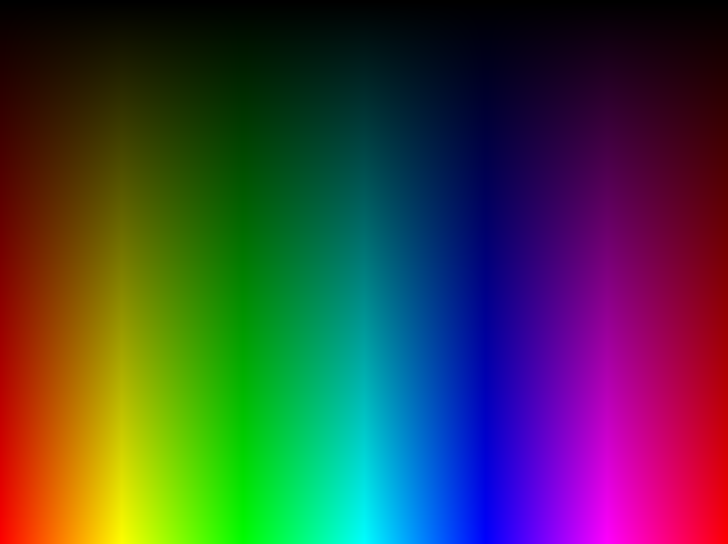
\includegraphics[width=.8\textwidth]{../photos/original_rainbow}
        \caption[originalRainbow]{Original rainbow image}
        \label{fig:original_rainbow}
    \end{subfigure}%
    \begin{subfigure}{.5\textwidth}
        \centering
        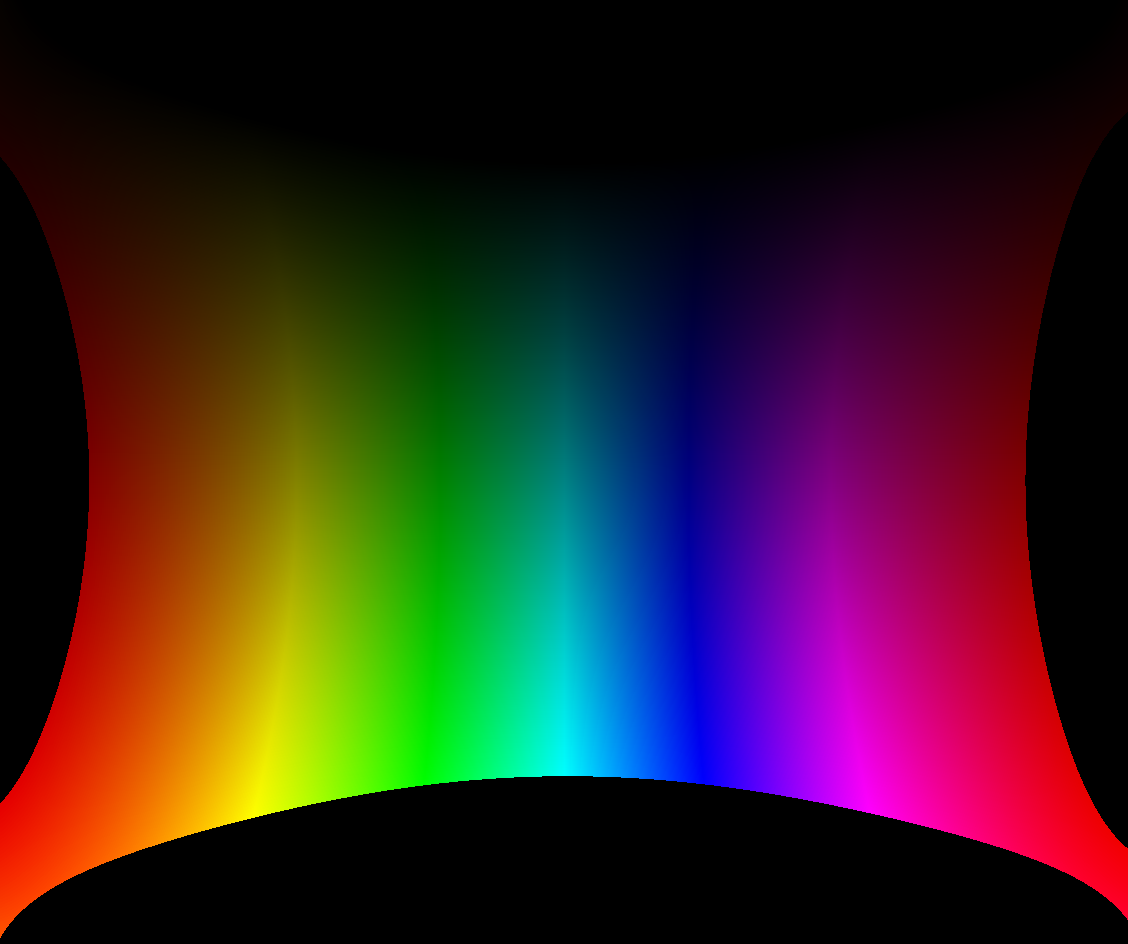
\includegraphics[width=.8\textwidth]{../photos/undistorted_rainbow}
        \caption[originalRainbow]{Undistorted rainbow image}
        \label{fig:undistorted_rainbow}
    \end{subfigure}
    \caption{Undistorted rainbow image}
    \label{fig:original_undistorted_rainbow}
\end{figure}
The undistorted image~\ref{fig:undistorted_rainbow} is larger than the original rainbow image~\ref{fig:original_rainbow}, that is because some pixel are moved out of the original image bounds because the camera can see "further" at the corners than at the sides.
This effect can also be seen in some example footage of the table:
\begin{figure}[H]
    \centering
    \begin{subfigure}{.5\textwidth}
        \centering
        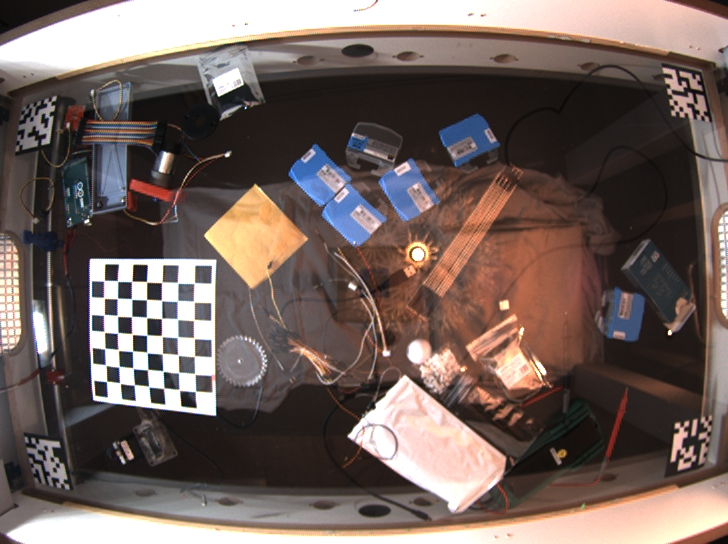
\includegraphics[width=.8\textwidth]{../photos/original_example8}
        \caption[originalRainbow]{Original image}
        \label{fig:original_example8}
    \end{subfigure}%
    \begin{subfigure}{.5\textwidth}
        \centering
        \includegraphics[width=.8\textwidth]{../photos/output8}
        \caption[originalRainbow]{Undistorted image}
        \label{fig:undistorted_example8}
    \end{subfigure}
    \caption{Undistorted example image}
    \label{fig:original_undistorted_example}
\end{figure}
Therefore we have to crop the image at the sides by a different amount, I made a simple graphical user interface (GUI) to adjust the cropping values.
The GUI can be seen here:
\begin{figure}[H]
    \centering
    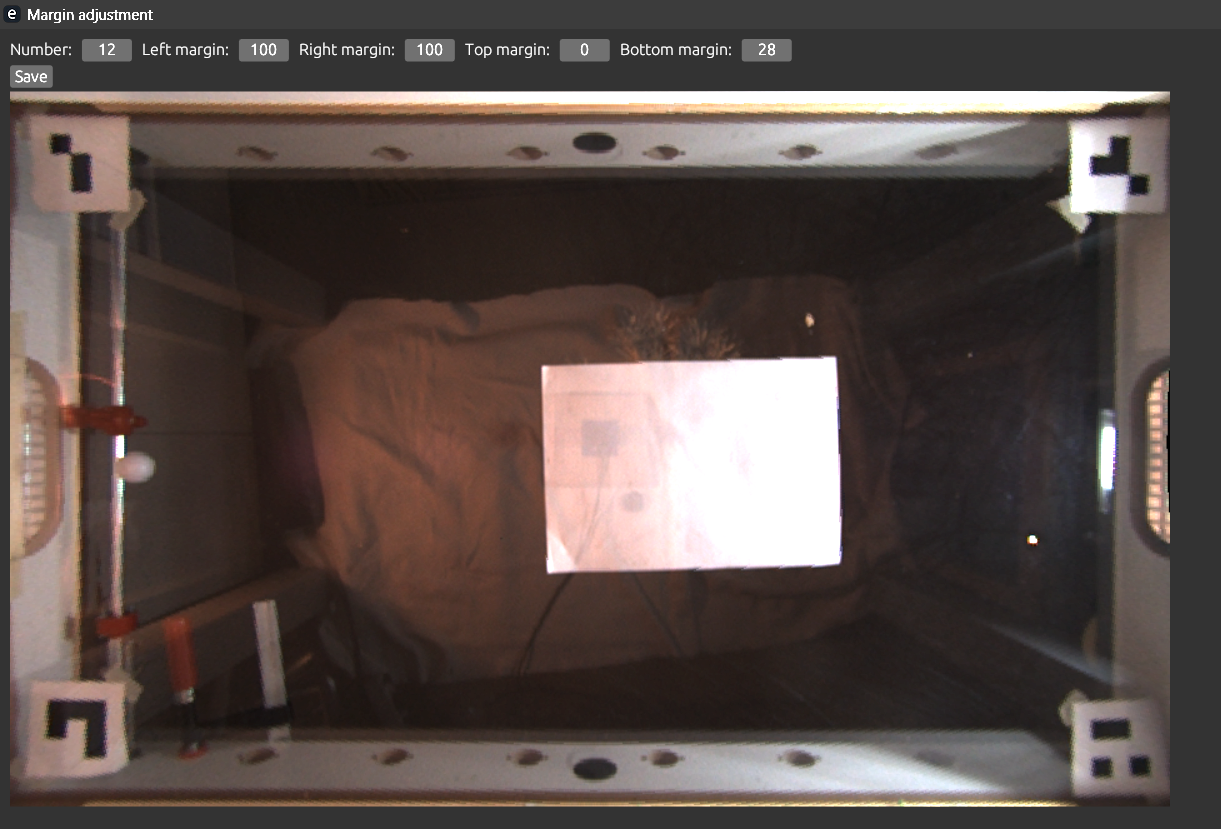
\includegraphics[width=0.8\textwidth]{../photos/margin_adj_gui}
    \caption[marginadjgui]{Margin Adjustment GUI}
    \label{fig:margin_adj_gui}
\end{figure}
The GUI is also written in rust using the egui\autocite{egui} library.
\todo{Fix the egui cite command (numbers instead of name)}
The cropped example image looks like this:
\begin{figure}[H]
    \centering
    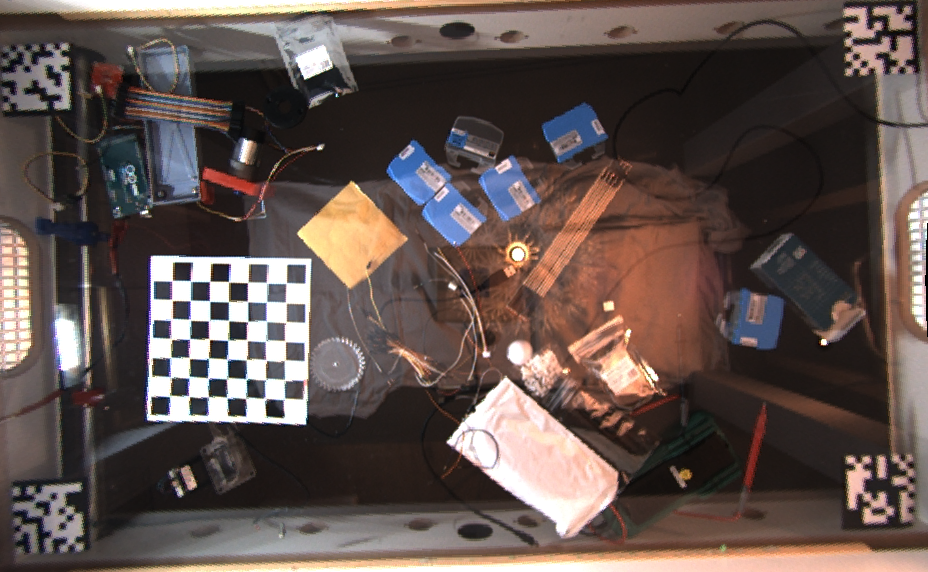
\includegraphics[width=0.8\textwidth]{../photos/example8_cropped}
    \caption[croppedexampleimage]{Cropped example image}
    \label{fig:example8_cropped}
\end{figure}

\subsection{Real World Coordinates}\label{subsec:real-world-coordinates}
An important part of the software is to convert the pixel coordinates to real-world coordinates.
This is done by adding fiducials (markers that are known to be at a specific position) to the table.
The fiducials are placed at the corners of the table, and the coordinates are measured in millimeters.
They can be seen here:
\begin{figure}[H]
    \centering
    \begin{subfigure}{.2\textwidth}
        \centering
        \fbox{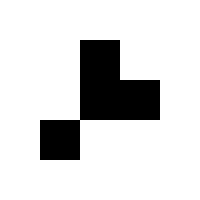
\includegraphics[width=.7\textwidth]{../photos/fiducials/fiducial_1}}
        \caption[originalRainbow]{Fiducial 1}
        \label{fig:fid_1}
    \end{subfigure}%
    \begin{subfigure}{.2\textwidth}
        \centering
        \fbox{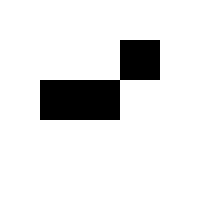
\includegraphics[width=.7\textwidth]{../photos/fiducials/fiducial_2}}
        \caption[originalRainbow]{Fiducial 2}
        \label{fig:fid_2}
    \end{subfigure}
    \begin{subfigure}{.2\textwidth}
        \centering
        \fbox{
\includegraphics[width=.7\textwidth]{../photos/fiducials/fiducial_3}}
        \caption[originalRainbow]{Fiducial 3}
        \label{fig:fid_3}
    \end{subfigure}
    \begin{subfigure}{.2\textwidth}
        \centering
        \fbox{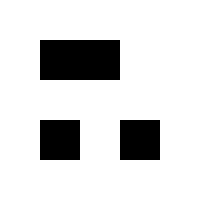
\includegraphics[width=.7\textwidth]{../photos/fiducials/fiducial_4}}
        \caption[originalRainbow]{Fiducial 4}
        \label{fig:fid_4}
    \end{subfigure}
    \caption{Fiducials}
    \label{fig:fiducials_all}
\end{figure}
To calibrate the real world coordinates one has to detect the fiducials reliably in the image.
This can be done by using a convolutional neural network (CNN) to detect the fiducials.

\subsubsection{Training Data}\label{subsubsec:training-data}
To train the CNN, one needs a lot of images containing the fiducials, making such a lot of images and then checking where exactly the coordinates of the midpoint of the fiducial lies is very tedious and not practical.
Therefore i wrote a Java programm to generate about 250 labeled images to train the CNN.
An image containing all the fiducials looks like this (the red point shows the midpoint of the fiducial):
\begin{figure}[H]
    \centering
    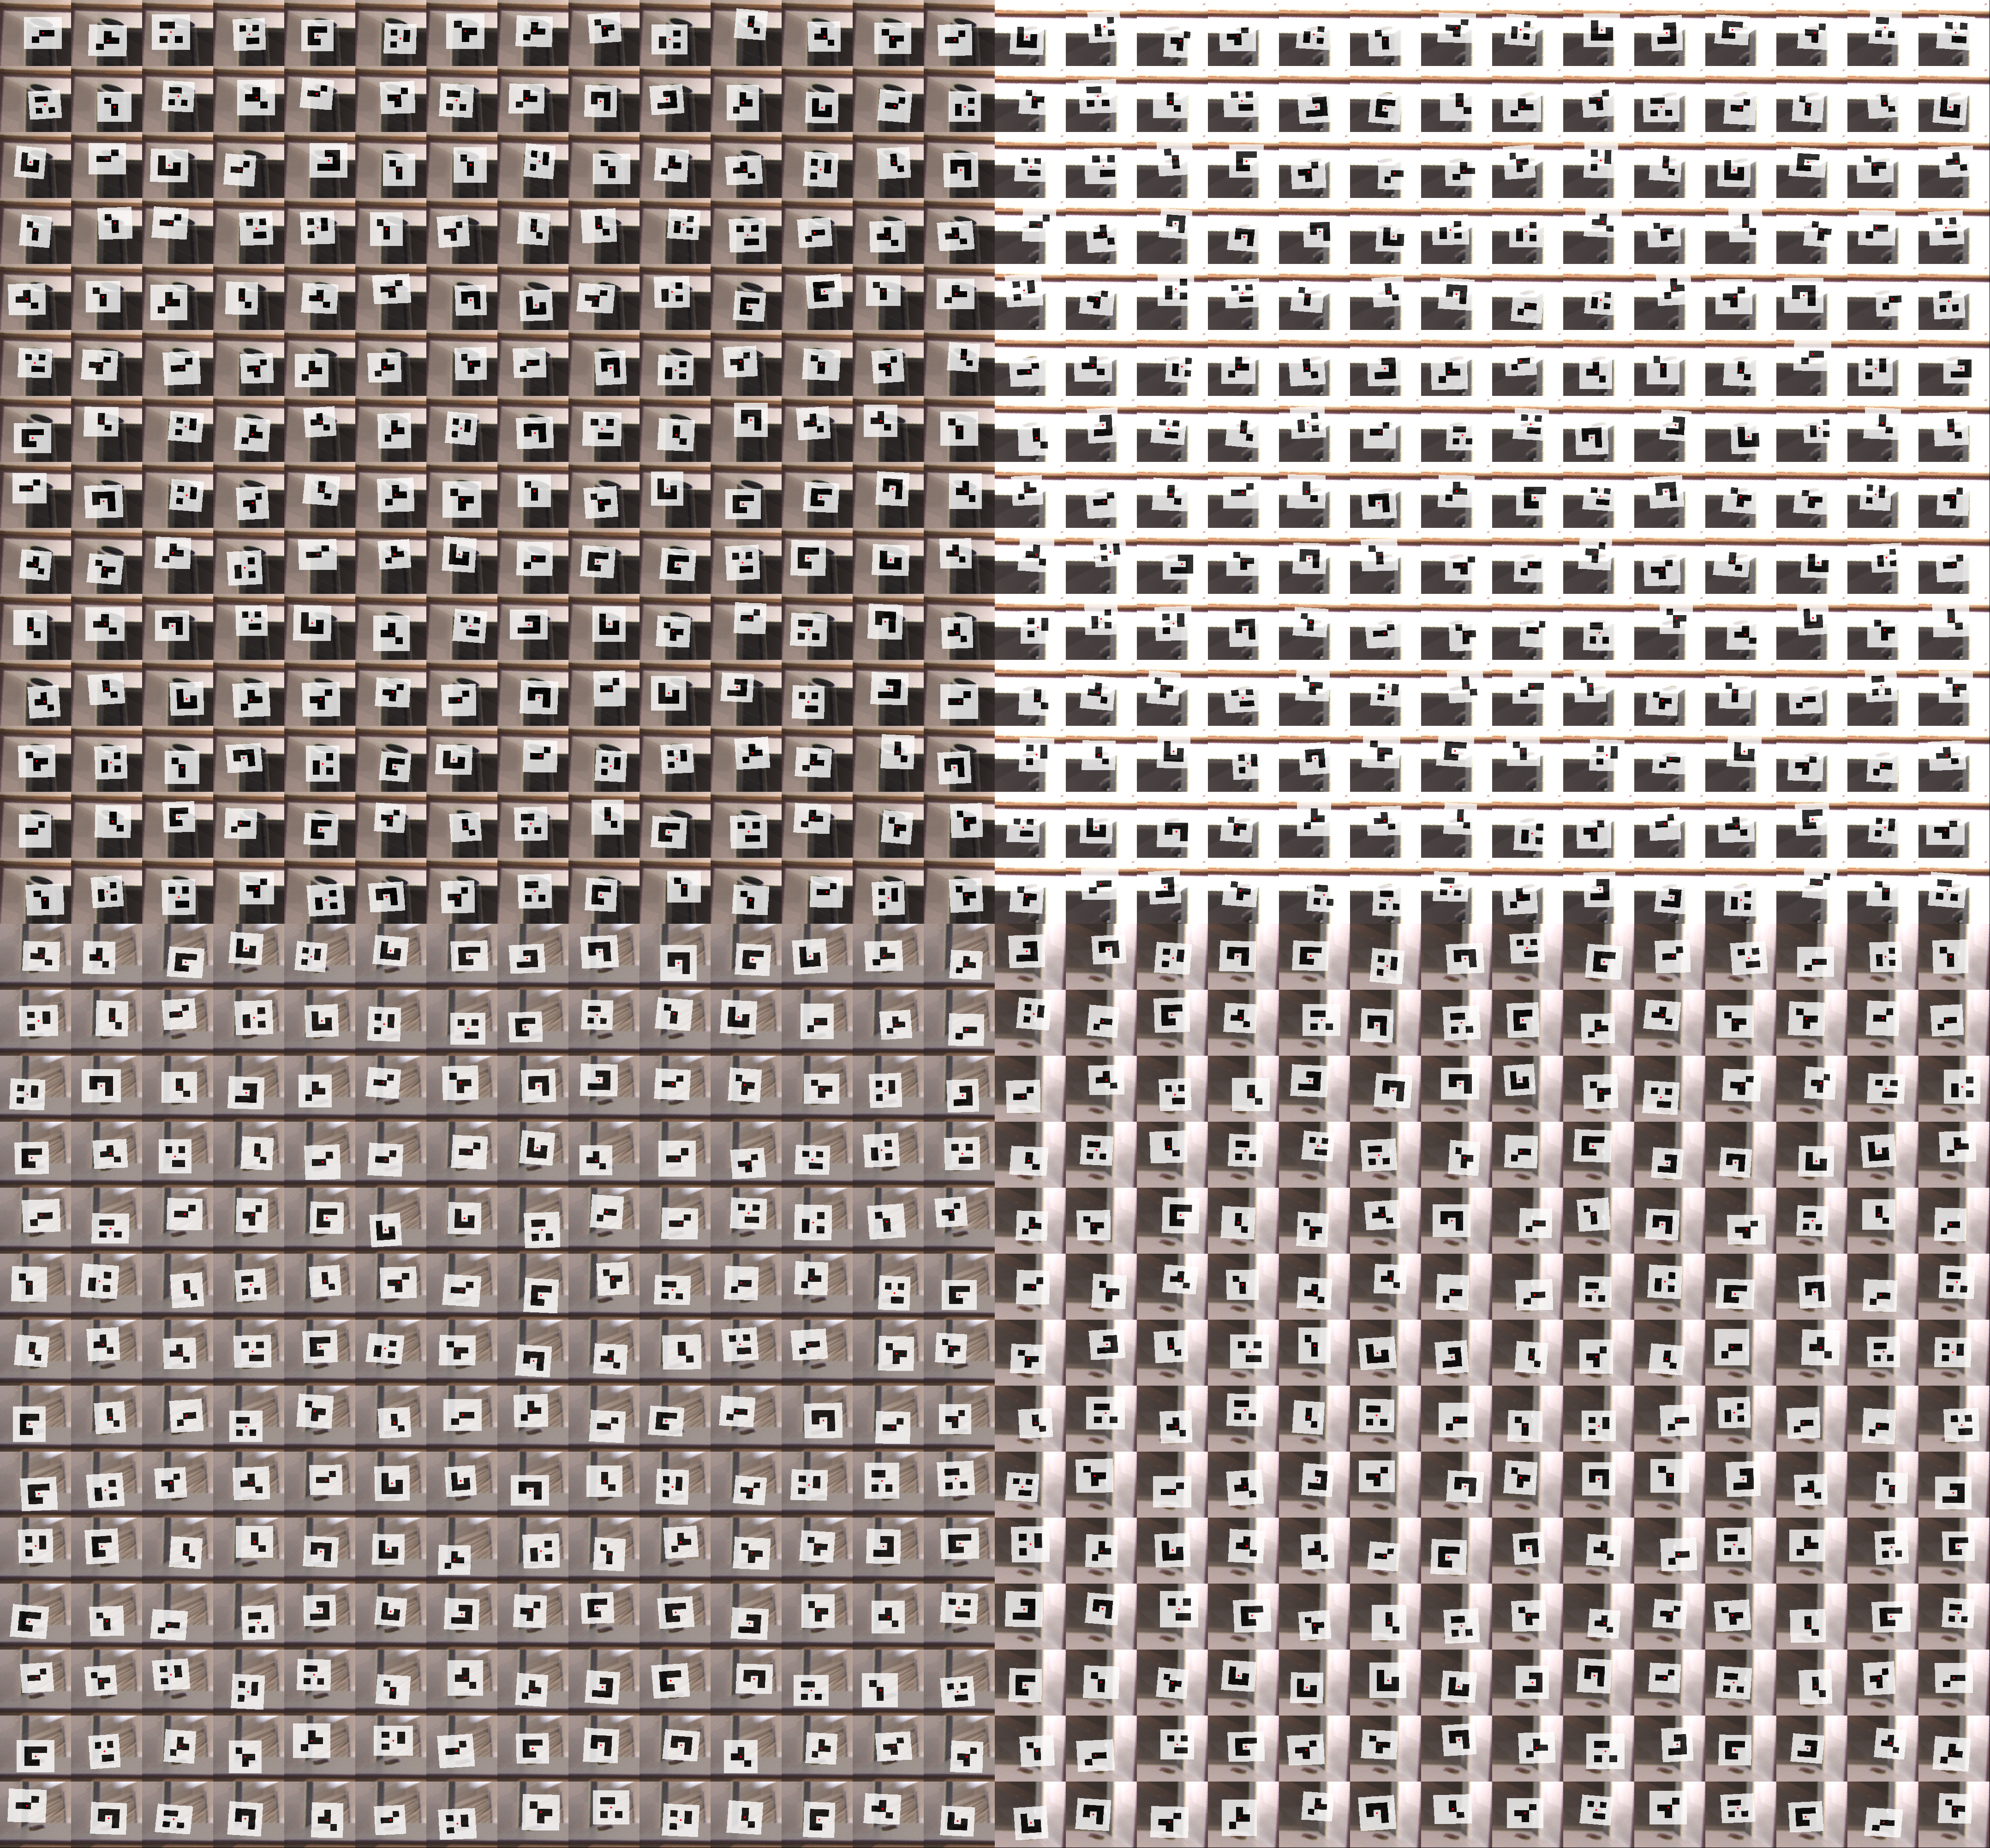
\includegraphics[width=0.8\textwidth]{../photos/training_whole_general_image}
    \caption[fiducials]{Training fiducials}
    \label{fig:fiducials}
\end{figure}
The trick I am using is that I know that the fiducials always lie in the corners of the table, so I can generate the images by just placing the fiducials in the corners with some random offset.
The different parts can be seen here:

\begin{figure}[H]
    \centering
    \begin{tikzpicture}
        % Include the image
        \node[anchor=south west, inner sep=0] (image) at (0,0) {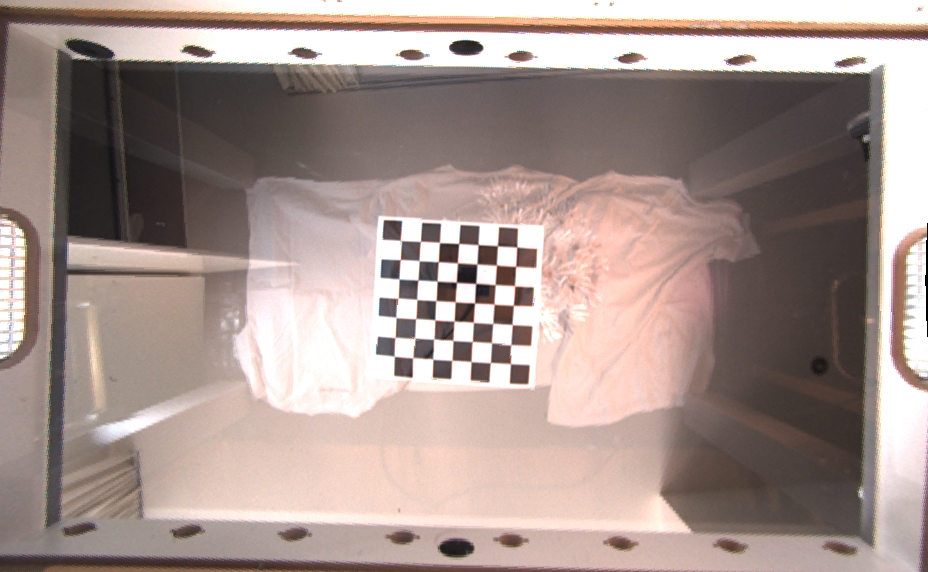
\includegraphics[width=0.8\textwidth]{../photos/base_img}};
        \begin{scope}
            [x={(image.south east)}, y={(image.north west)}]
            % vertical lines (6 parts)
            \foreach \i in {1/6, 2/6, 3/6, 4/6, 5/6} {
                \draw[red, very thick] (\i, 0) -- (\i, 1);
            }
            % horizontall lines (4 parts)
            \foreach \i in {1/4, 2/4, 3/4} {
                \draw[red, very thick] (0, \i) -- (1, \i);
            }
        \end{scope}
    \end{tikzpicture}
    \caption{Image split into 4 horizontal and 6 vertical parts}\label{fig:figure}
\end{figure}
\textbf{Create and Train the CNN}\\
I made two separate CNNs, one for detecting the fiducial (number from 1-4 as there are four fiducials) (also known as classification) and one for detecting the coordinate of the midpoint of the fiducial (from where the real-world measurements are made).
The CNNs are trained using the tensorflow library made by google.
The structure of the CNNs can be seen here:
\begin{figure}[H]
    \centering
    \begin{subfigure}{.5\textwidth}
        \centering
        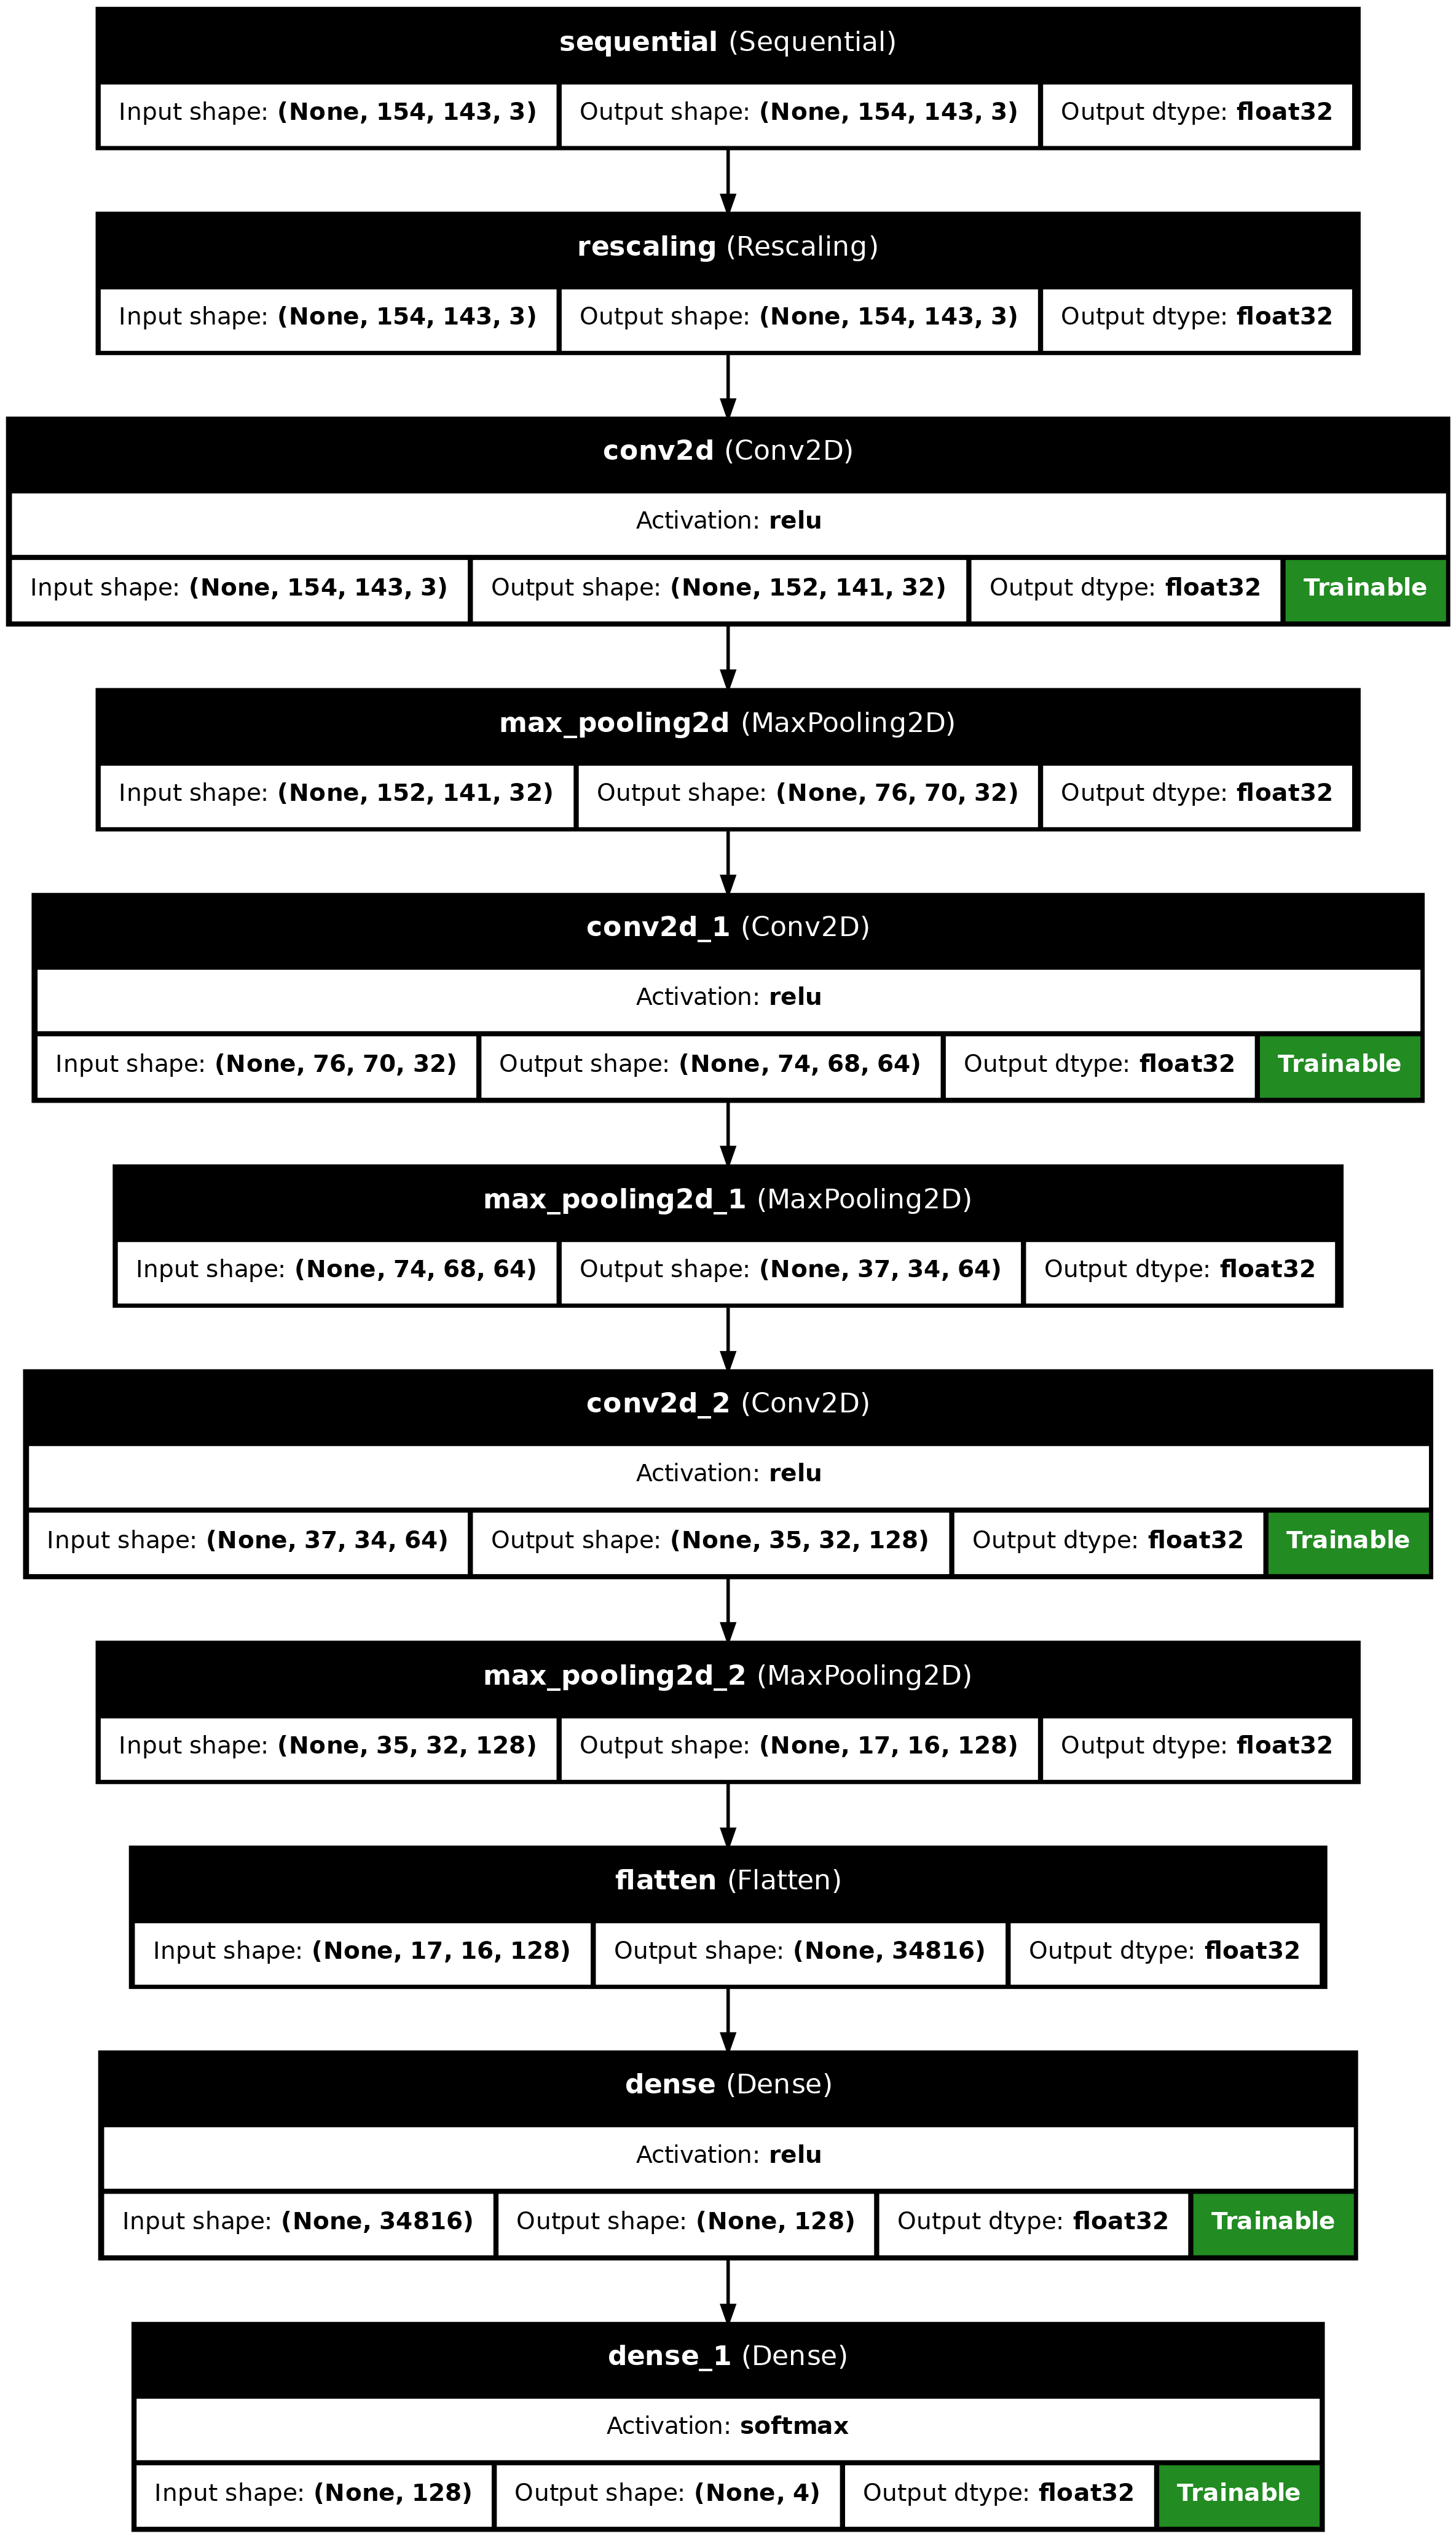
\includegraphics[width=.8\textwidth]{../photos/fiducial_classifier_model}
        \caption[originalRainbow]{Fiducial classifier model}
        \label{fig:fiducial_classifier_model}
    \end{subfigure}%
    \begin{subfigure}{.5\textwidth}
        \centering
        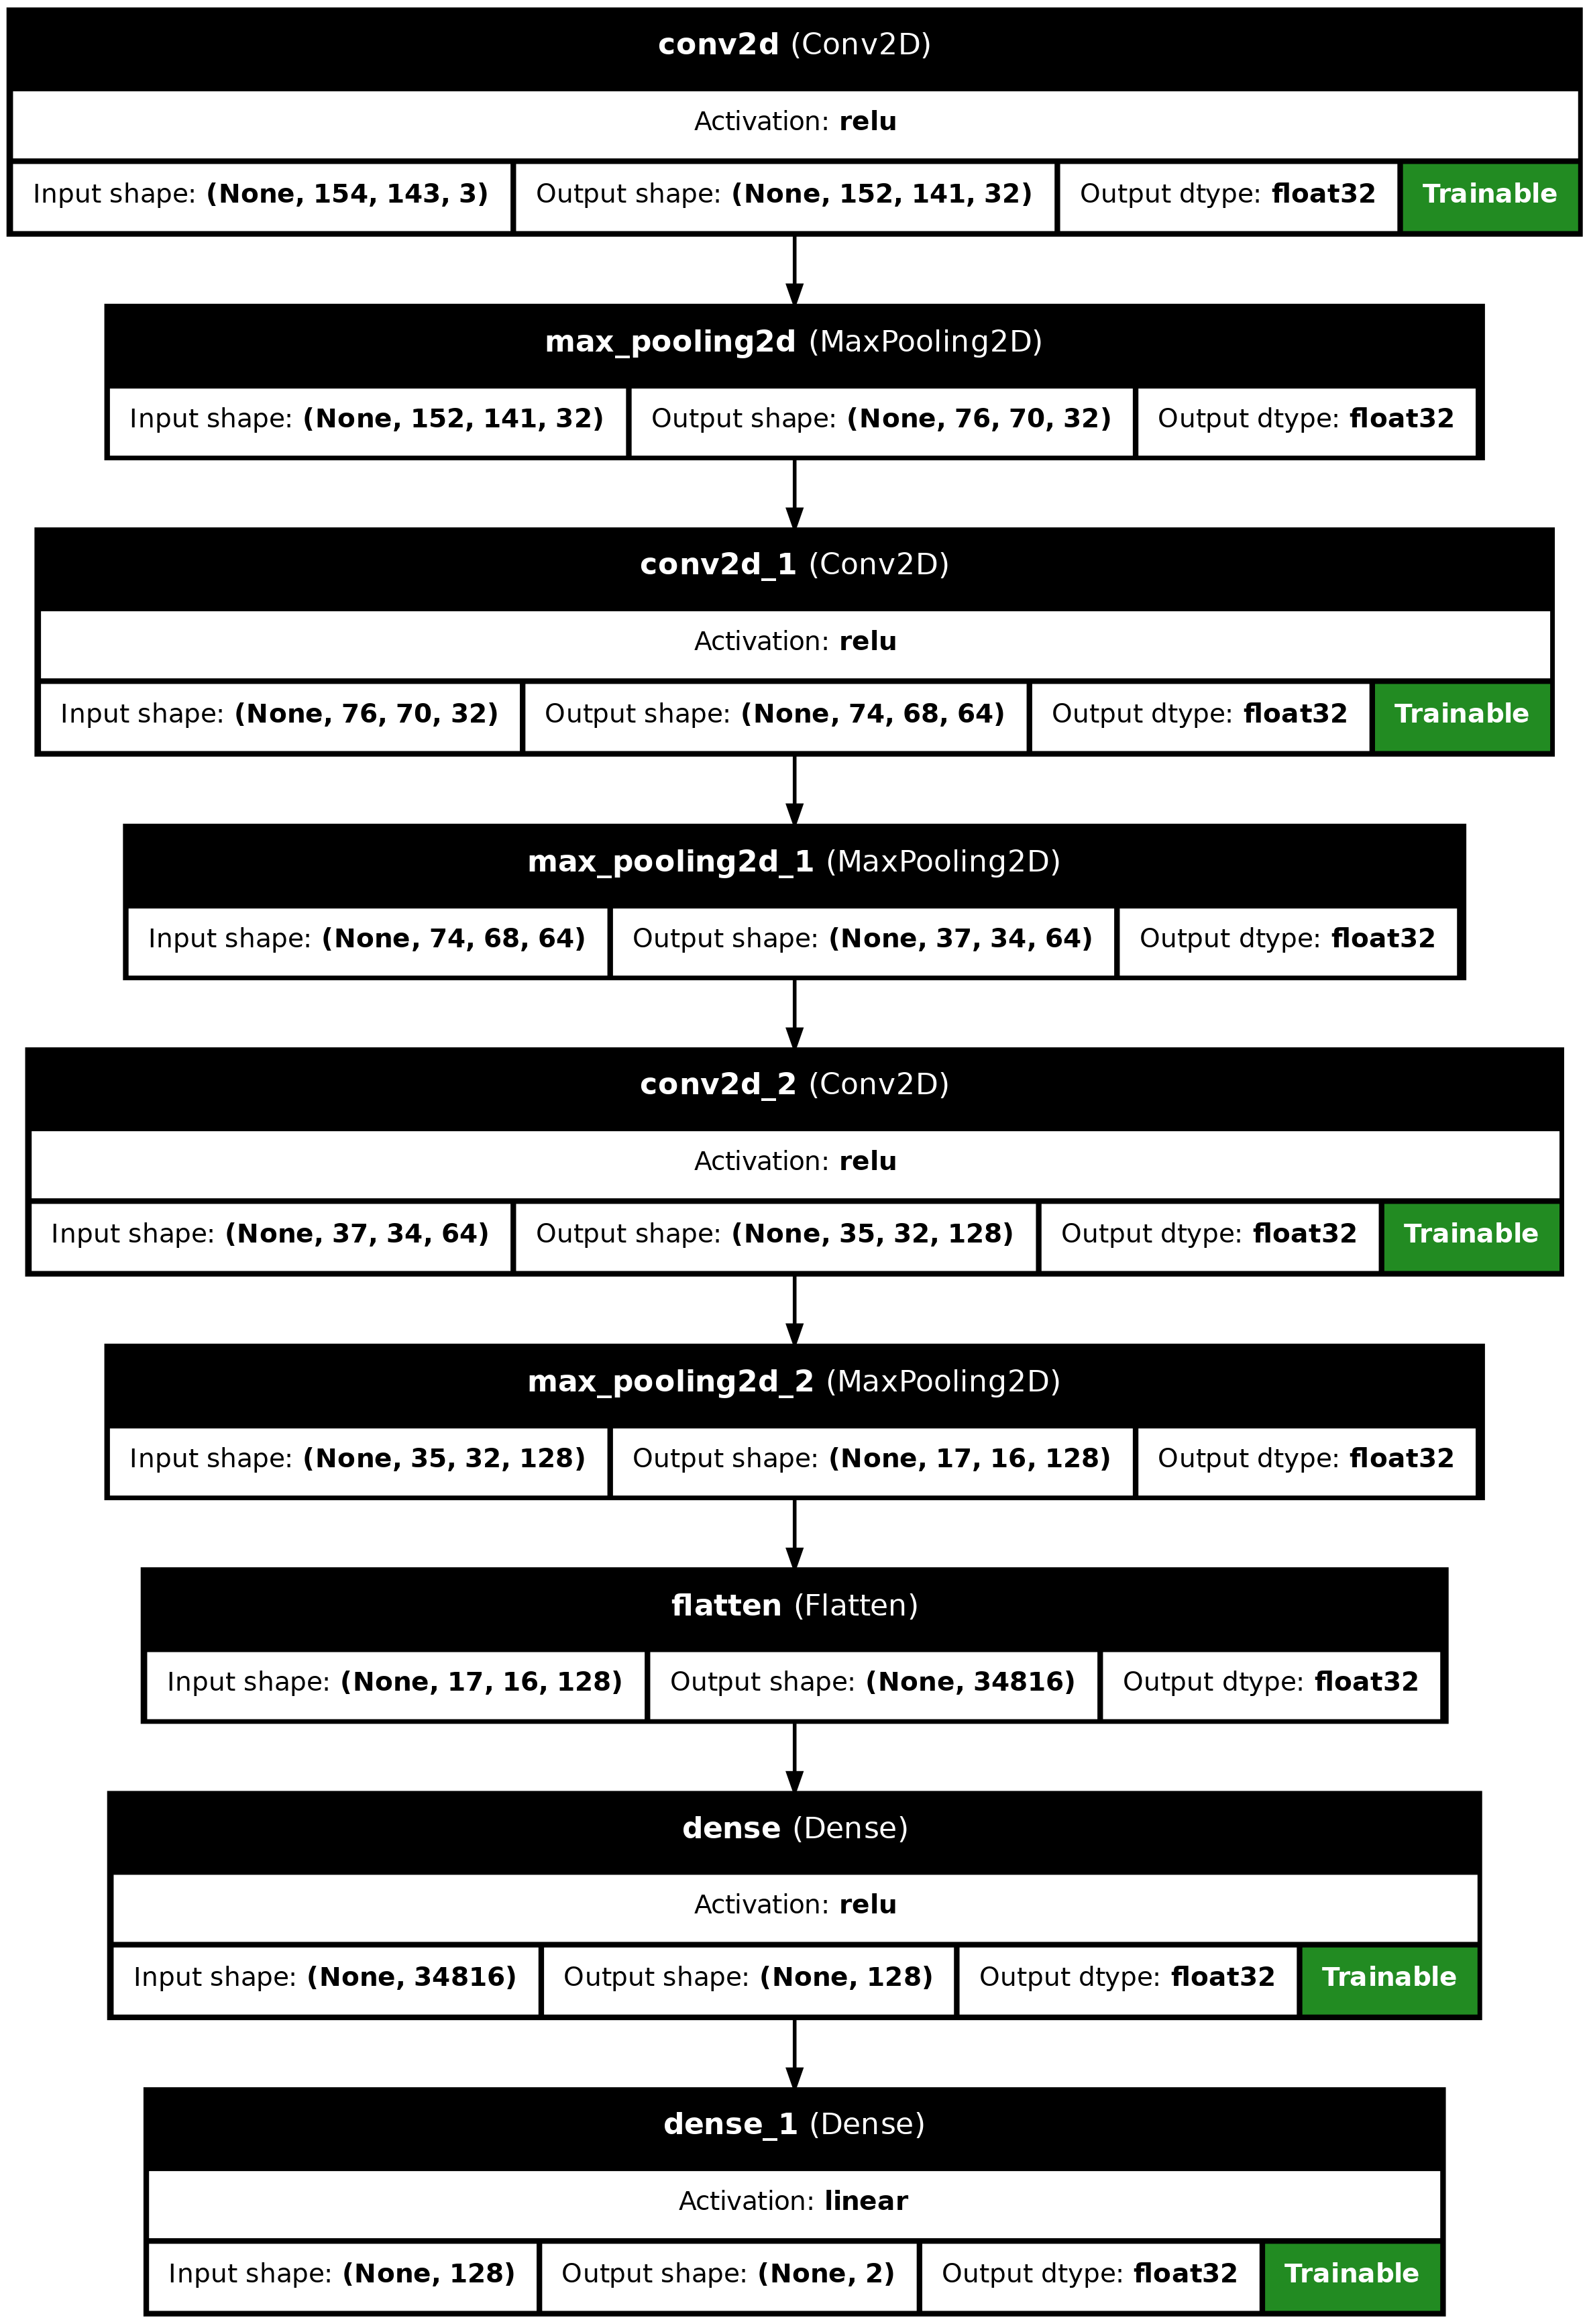
\includegraphics[width=.8\textwidth]{../photos/fiducial_coords_model}
        \caption[originalRainbow]{Fiducial coordinates model}
        \label{fig:fiducial_coords_model}
    \end{subfigure}
    \caption{Structure of the CNNs}
    \label{fig:CNN_structure}
\end{figure}
An interesting way to visualize the way the CNN works is to use gradcam to visualize the gradient of the image, which corresponds to the parts of the image the CNN is looking at.
\begin{figure}[H]
    \centering
    \includegraphics[width=0.9\textwidth]{../photos/gradcam_combined_image}
    \caption[cnn-gradcam]{Gradcam of the different layers (using another CNN which was trained to do the same task)}
    \label{fig:gradcam_combined_image}
\end{figure}

% Todo add stats about the real world training/tests
\todo{Todo add stats about the real world training/tests}


\section{Ball Detection}\label{sec:ball-detection}
The ball detection is a crucial part of the software, because if the ball is not detected correctly, the whole system will not work.
To detect ball an image is taken without the ball present and then the image with the ball is subtracted from the image without the ball, so that only the ball remains in the image.
But a problem that arises is that also other things that change are detected, like people moving or the table moving.
Luckily the glass table is so reflective and the light from the bottom is strong enough that the people behind the glass table have a low contrast in the image, so they are not detected.
To detect the ball I just filter out the white pixels in the image, because the ball is white.
The ball detection can be seen here:
\begin{figure}[H]
    \centering
    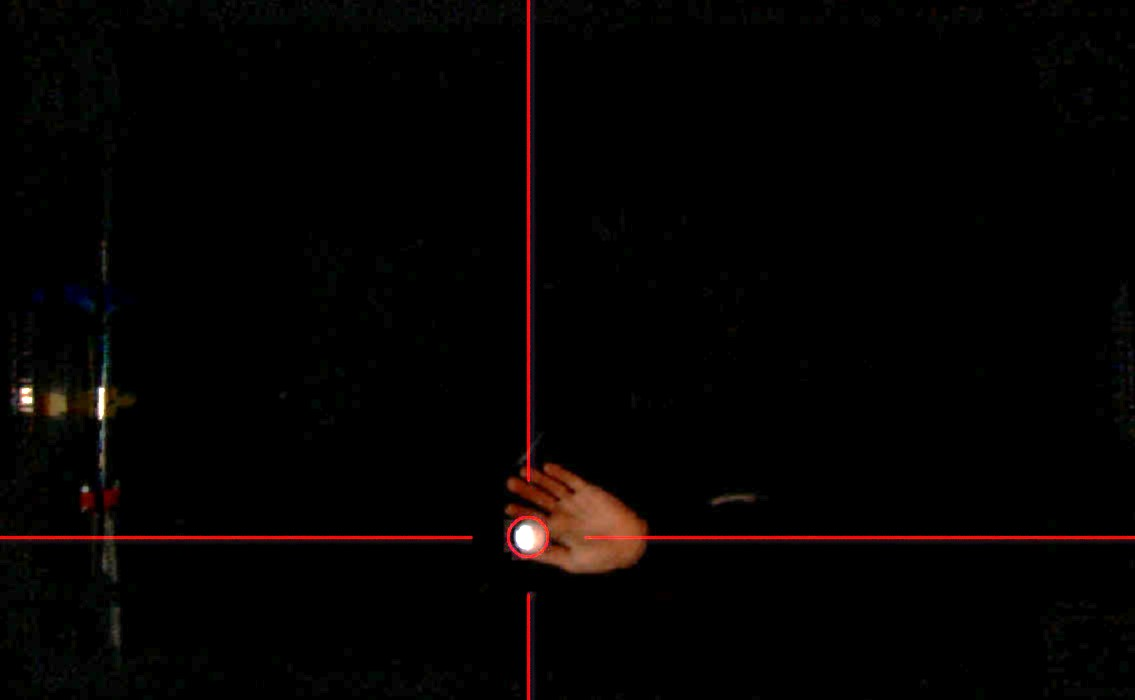
\includegraphics[width=0.9\textwidth]{../photos/ball_detection}
    \caption[ball-detection]{Ball detection in action}
    \label{fig:ball_detection}
\end{figure}
But having the pixel coordinates is not very useful, so we have to convert the pixel coordinates to real-world coordinates.
To compute the real world coordinates we compare the pixel coordinates of the ball to the pixel coordinates of the fiducials.
I measured the distance between the walls and the fiducials and made a coordinate system so that the fiducial with the number 2 lies in the top left corner (0,0) and the other fiducials are placed accordingly.
Then to compute the real world coordinates I use a homography matrix to transform the pixel coordinates to real world coordinates.
\section*{Homography Calculation}

Homography is used to map points from image coordinates to real-world coordinates.
The transformation is defined as:

\begin{equation}
    \begin{bmatrix}
        x' \\
        y' \\
        1
    \end{bmatrix}
    = H \cdot
    \begin{bmatrix}
        x \\
        y \\
        1
    \end{bmatrix}\label{eq:homography}
\end{equation}

Where:
\begin{itemize}
    \item \( (x, y) \) are the pixel coordinates,
    \item \( (x', y') \) are the real-world coordinates,
    \item \( H \) is the \( 3 \times 3 \) homography matrix.
\end{itemize}

In Python, we compute \( H \) using the $cv2.findHomography$ function:

%\begin{lstlisting}[language=python,breaklines,label={lst:python_homography}]
%homography_matrix, _ = cv2.findHomography(pixel_points, real_points)
%\end{lstlisting}

\[
    H, \text{\_} = \text{cv2.findHomography}(\text{pixel\_points}, \text{real\_points})
\]
% todo: should i explain how the homography matrix is calculated?
\todo{Should i explain how the homography matrix is calculated?}

In Rust, this matrix is applied to new pixel points via matrix multiplication and normalization.
% todo: should i explain that i save the stuff a file and then read it to save time?


\section{Prediction}\label{sec:prediction}
To predict where the ball will go in the future I use a simple linear regression model.
But first I have to check whether the ball is still flying into the same direction and with the same velocity.
This is done by using the last position and computing the current position with the current velocity.
If the difference between the prediction and the the real world position is too large then I delete the positions and start over.
\begin{figure}[H]
    \centering
    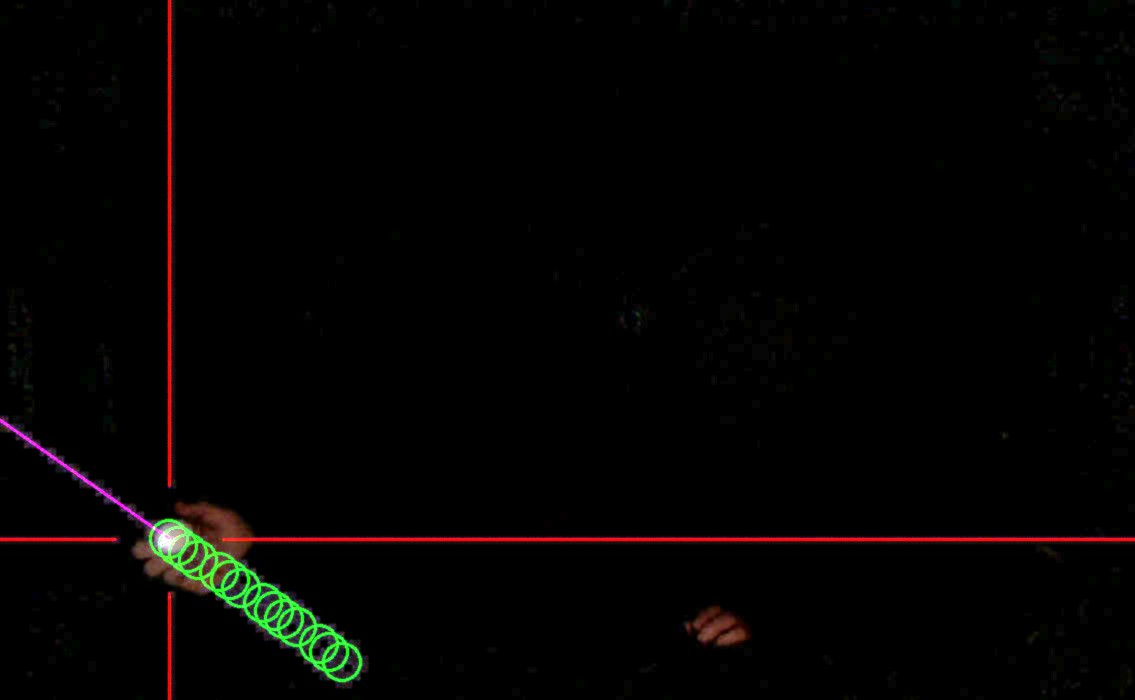
\includegraphics[width=0.9\textwidth]{../photos/ball_prediction}
    \caption[ball-prediction]{Prediction of the future positions of the ball. The green balls are the last positions and the violet line is the current velocity}
    \label{fig:ball_prediction}
\end{figure}

% todo: should i explain the linear regression model and the linear algebra behind it?
\todo{Should i explain the linear regression model and the linear algebra behind it?}
To find out where the ball will end up when it reaches the goalkepper (or any player), I can just compute the intersection between the line of the ball and the line of the goalkepper.
The line of the ball can be computed with the current position $\vec{r}$, the current velocity $\vec{v}$ and the player's $x$ coordinate.
\begin{equation}
    \begin{split}
        \vec{r} &= \begin{bmatrix}
                       x \\
                       y
        \end{bmatrix}\\
        \vec{v} &= \begin{bmatrix}
                       v_x \\
                       v_y
        \end{bmatrix}\\
%    let t = (x - self.position.x) / self.velocity.x;
%        Some(self.position + self.velocity * t)
        t &= \frac{x - r_x}{v_x}\\
        \vec{r}_\text{intersection} &= \vec{r} + \vec{v} \cdot t
    \end{split}\label{eq:ball_intersection}
\end{equation}
Now we only have to convert the $\vec{r}_\text{intersection}$ to real world coordinates and we have the position where the ball will end up, which we send to the arduino to move the stepper motor to this position.


\section{Controlling the motors}\label{sec:controlling-the-motors}
To control the motors I use an Arduino Mega 2560, because it has enough pins to control all the motors at once.
The Arduino is connected to the computer via USB, and the computer sends the motor positions to the Arduino via serial communication.

\subsubsection{Controlling the DC-Motor}\label{subsubsec:controlling-the-dc-motor}
The DC-Motor is controlled by the stepper motor driver L298N as seen here\ref{ch:electronics}.




